% !TeX spellcheck = en_US
% !TeX root = notes.tex
\subsection{Network Layer}
\begin{itemize}
	\item transport segment from sending to receiving host
	\item on sending side encapsulates segments into datagrams
	\item on receiving side, delivers segments to transport layer
	\item network layer protocols in \textbf{every} host, router
	\item router examines header fields in all IP datagrams passing through it
\end{itemize}
\subsubsection{Network Layer Functions}
\begin{description}
	\item[Forwarding:] move packets from router's input to appropriate router output
	\item[Routing:] determine route taken by packets from source to destination \textit{(routing algorithms)}
\end{description}
\subsubsection{Data Plane, Control Plane}
\textbf{Data Plane}
\begin{itemize}
	\item local, per-router function
	\item determines how datagram arriving on router input port is forwarded to router output port
	\item forwarding function
\end{itemize}
\textbf{Control plane}
\begin{itemize}
	\item network-wide logic
	\item determines how datagram is routed among routers along end-end path from source host to destination host
	\item two control-plane approaches:
	\begin{description}
		\item[Traditional Routing Algorithms:] implemented in routers
		\item[Software-defined networking (SDN):] implemented in (remote) servers
	\end{description}
\end{itemize}

\subsection{Router Forwarding}
\begin{description}
	\item[Destination-based forwarding:] forward based only on destination IP address (traditional)
	\item[Generalized forwarding:] forward based on any set of header field values
\end{description}
\subsubsection{Destination-based forwarding}
A link interface is assigned to a range of destination address ranges\\
\begin{note}{Longest Prefix Matching}
	When looking for forwarding table entry for given destination address, use \textbf{longest} address prefix that matches destination address. Longest prefix matching: often performed using ternary content addressable memories (TCAMs). Cisco Catalyst can hold up $\approx$1M routing table entries in TCAM.
\end{note}
\begin{description}
	\item[Content Addressable:] present address to TCAM; retrieve address in one clock cycle, regardless of table size
\end{description}
\subsubsection{Switching Fabrics}
\begin{itemize}
	\item transfer packet from input buffer to appropriate output buffer
	\item switching rate: rate at which packets can be transfered from inputs to outputs (often measured as multiple of input/output line rate, $N$ inputs: switching rate $N$ times line rate desirable)
	\item three types of switching fabrics
\end{itemize}
\begin{figure}[H]
	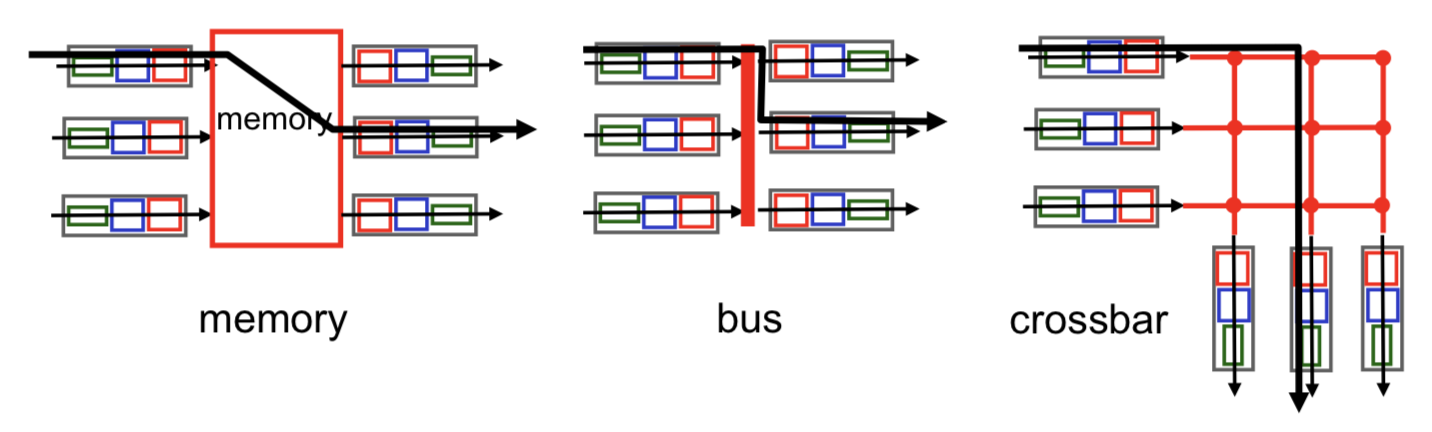
\includegraphics[width=\linewidth]{switching}
	\centering
	\caption{Different Types of Switching Fabrics}
\end{figure}
\textbf{Switching via Memory}
\begin{itemize}
	\item traditional computes with switching under direct control of CPU
	\item packet copied to system's memory
	\item speed limited memory bandwidth (2 bus crossing per datagram)
\end{itemize}
\textbf{Switching via a Bus}
\begin{itemize}
	\item datagram from input port memory to output port memory via a shared bus
	\item \textbf{bus contention:} switching speed limited by bus bandwidth
	\item 32 Gbps bus, Cisco 5600: sufficient speed for access and enterprise routers
\end{itemize}
\textbf{Switching via Interconnection Network}
\begin{itemize}
	\item overcome bus bandwidth limitations
	\item banyan networks, crossbar, other interconnection nets initially developed to connect processors in multiprocessor
	\item advanced design: fragmenting datagram into fixed length cells, switch cells through the fabric
	\item Cisco 12000: switches 60 Gbps through the interconnection network
\end{itemize}
\subsubsection{Input port queuing}
\begin{itemize}
	\item fabric slower than input ports combined $\rightarrow$ queuing may occur at input queues (queuing delay and loss due to input buffer overflow)
	\item \textbf{Head-of-the-Line (HOL) blocking:} queued datagram at front of queue prevents others in queue from moving forward
\end{itemize}
\subsubsection{Output ports}
\begin{itemize}
	\item \textbf{Buffering} required from fabric faster rate (Datagram (packets) can be lost due to congestion, lack of buffers)
	\item \textbf{Scheduling} datagrams (Priority scheduling -- who gets best performance, network neutrality)
\end{itemize}
\begin{note}{How much buffering?}
	RFC 3439 rule of thumb: average buffering equal to ``typical'' RTT (say 250 msec) times link capacity C (e.g. C = 10 Gbps link, 2.5 Gbit buffer). Recent recommendation with $N$ flows, buffering equal to $$\frac{RTT\times C}{\sqrt{N}}$$
\end{note}
\subsubsection{Scheduling Mechanisms}
\begin{description}
	\item[Scheduling:] choose next packet to send on link
	\item[FIFO scheduling:] send in order of arrival to queue
	\begin{description}
		\item[discard policy:] if packet arrives to full queue, who to discard
		\begin{description}
			\item[tail drop:] drop arriving packet
			\item[priority:] drop/remove on priority basis
			\item[random:] drop/remove randomly
		\end{description}
	\end{description}
	\item[priority scheduling:] send highest priority queued packet. Multiple \textit{classes}, with different priorities (class may depend on marking or other header info, e.g. IP source/dest, port number, etc)
	\item[RR scheduling:] multiple classes. Cyclically scan class queues, sending one complete packet from each class (if available)
	\item[WFQ scheduling:] generalized Round Robin. Each class gets weighted amount of service in each cycle
\end{description}

\subsection{IP}\label{sec:ip}
\subsubsection{IP Datagram Format}
\begin{figure}[H]
	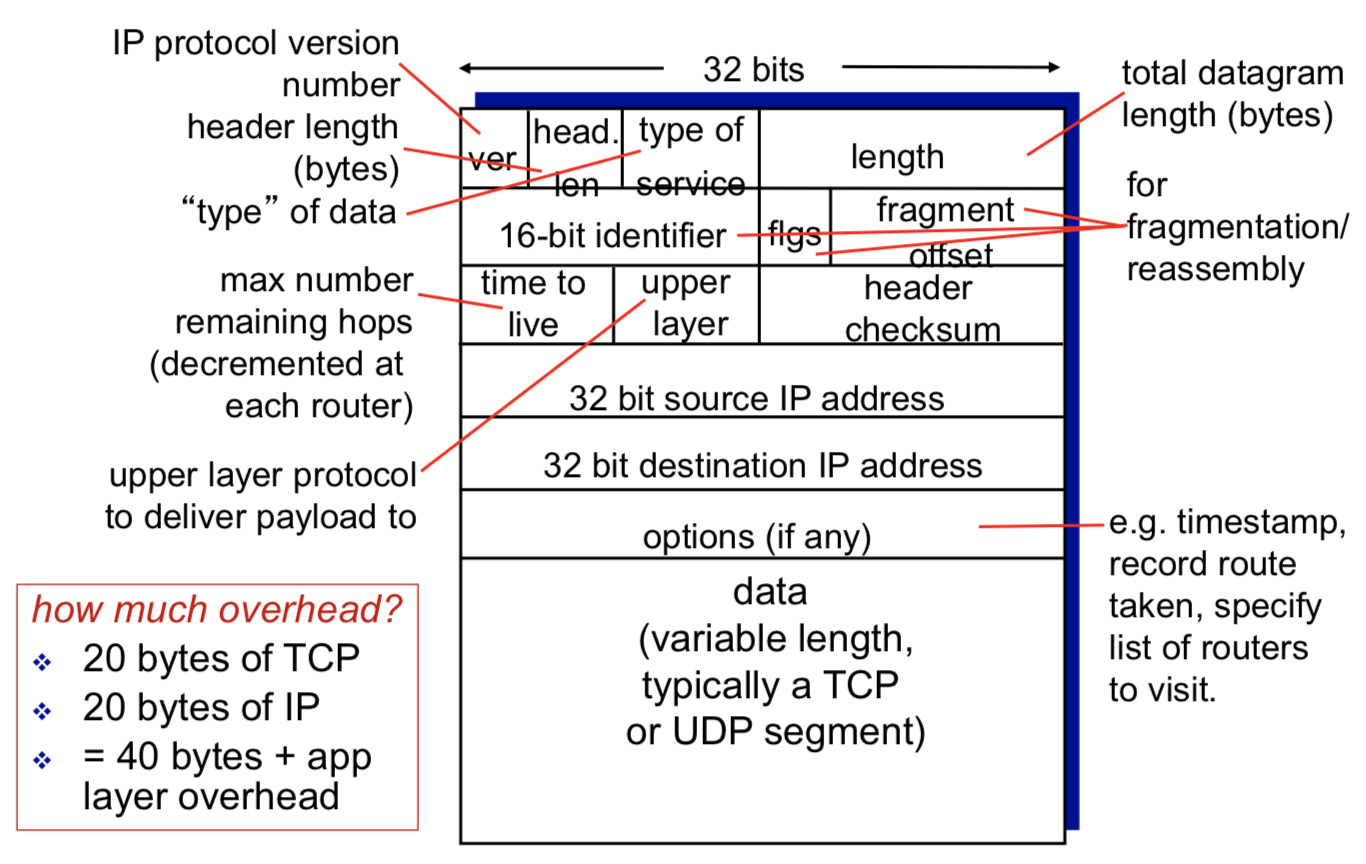
\includegraphics[width=\linewidth]{ip}
	\centering
	\caption{IP Datagram Format}
\end{figure}
\subsubsection{IP Fragmentation, Reassembly}
Large IP datagram divided (``fragmented'') within net
\begin{itemize}
	\item one datagram becomes several datagrams
	\item ``reassembled'' only at final datagrams
	\item IP header bits used to identify, order related fragments
\end{itemize}
\subsubsection{IP Addressing}
\begin{description}
	\item[IP Address:] 32-bit identifier for host, router interface
	\item[interface:] connection between host/router and physical link. Router's typically have multiple interfaces
\end{description}
\subsubsection{Subnets}
\textbf{Subnet part} -- high order bits. \textbf{Host part} -- low order bits
\begin{itemize}
	\item device interfaces with same subnet part of IP address
	\item can physically reach each other \textbf{without intervening router}
	\item to determine the subnets, detach each interface from its host or router, creating islands of isolated networks
	\item each isolated network is called a \textbf{subnet}
\end{itemize}
CIDR: Classless InterDomain Routing
\begin{itemize}
	\item subnet portion of address of arbitrary length
	\item address format: \texttt{a.b.c.d/x}, where \texttt{x} is \# bits in subnet portion of address
\end{itemize}
\subsubsection{DHCP: Dynamic Host Configuration Protocol}\label{sec:dhcp}
\begin{leftbar}
	\textbf{Goal:} allow host to \textit{dynamically} obtain its IP address from network server when it joins network
\end{leftbar}
\begin{itemize}
	\item can renew its lease on address in use
	\item allows reuse of addresses (only hold address while connected)
	\item support for mobile users who want to join network (more shortly)
\end{itemize}
DHCP overview:
\begin{itemize}
	\item host broadcasts ``DHCP discover'' msg \textit{[optional]}
	\item DHCP server responds with ``DHCP offer'' msg \textit{[optional]}
	\item host requests IP address: ``DHCP request'' msg
	\item DHCP server sends address: ``DHCP ack'' msg
\end{itemize}
DHCP can return more than just allocated IP address on subnet:
\begin{itemize}
	\item address of first-hop router for client
	\item name and IP address of DNS server
	\item network mask (indicating network versus host portion of address)
\end{itemize}
\subsubsection{ICANN}\label{sec:icann}
\begin{itemize}
	\item allocates addresses
	\item manages DNS
	\item assigns domain names, resolves disputes
\end{itemize}
\subsubsection{NAT}\label{sec:nat}
All datagrams \textbf{leaving} local network have \textbf{same} single source NAT IP address
\begin{leftbar}
	\textbf{Motivation:} local network uses just one IP address as far as outside world is concerned
\end{leftbar}
\begin{itemize}
	\item range of addresses not needed from ISP: just one IP address for all devices
	\item can change addresses of devices in local network without notifying outside world
	\item can change ISP without changing addresses of devices in local network
	\item devices inside local net not explicity addressable, visible by outside world (a security plus)
\end{itemize}
\textbf{Implementation:} NAT router must
\begin{description}
	\item[Outdoing datagrams: replace] (source IP address, port \#) of every outgoing datagram to (NAT IP address, new port \#) ... remote clients/servers will respond using (NAT IP address, new port \#) as destination address
	\item[Remember (in NAT translation table)] every (source IP address, port \#) to (NAT IP address, new port \#) translation pair
	\item[Incoming datagrams: replace] (NAT IP address, new port \#) in destination fields of every incoming datagram with corresponding (source IP address, port \#) stored in NAT table
\end{description}
\begin{itemize}
	\item 16-bit port-number field: 60,000 simultaneous connections with a single LAN-side address
	\item NAT is controversial:
	\begin{itemize}
		\item routers should only process up to layer 3
		\item address shortage should be solved by IPv6
		\item violates end-to-end argument (NAT possibility must be taken into account by app designers, e.g. P2P applications)
		\item NAT traversal: what if client wants to connect to server behind NAT?
	\end{itemize}
\end{itemize}
\subsubsection{IPv6}\label{sec:ipv6}
\begin{leftbar}
	32-bit address space soon to be completely allocated
\end{leftbar}
Additionally:
\begin{itemize}
	\item header format helps speed processing/forwarding
	\item header changes to facilitate QoS
\end{itemize}
\textbf{IPv6 datagram format:}
\begin{itemize}
	\item fixed-length 40 byte header
	\item no fragmentation allowed
\end{itemize}
\subsubsection{IPv6 Datagram Format}
\begin{description}
	\item[Priority:] identify priority among datagrams in flow
	\item[Flow Label:] identify datagrams in same ``flow'' (concept of ``flow'' not well defined)
	\item[Next Header:] identify upper layer protocol for data
\end{description}
\begin{table}[H]
	\centering
	\caption{IPv6 Format}
	\begin{tabular}{cccc}
		\toprule
		\multicolumn{4}{c}{32 bits}\\
		\midrule
		version & pri & \multicolumn{2}{c}{flow label}\\
		\multicolumn{2}{c}{payload len} & next hdr & hop limit\\
		\multicolumn{4}{c}{source address (128 bits)}\\
		\multicolumn{4}{c}{destination address (128 bits)}\\
		\multicolumn{4}{c}{data}\\
		\bottomrule
	\end{tabular}
\end{table}
\subsubsection{Other changes from IPv4}
\begin{description}
	\item[checksum:] removed entirely to reduce processing time at each hop
	\item[options:] allowed, but outside of header, indicated by ``Next Header'' field
	\item[ICMPv6:] new version of ICMP (additional message types e.g. ``Packet Too Big'', multicast group management functions)
\end{description}
\subsubsection{Transition from IPv4 to IPv6}
\begin{itemize}
	\item not all routers can be upgraded simultaneously (no ``flag days'', how will network operate with mixed IPv4 and IPv6 routers)
	\item \textbf{tunneling:} IPv6 datagram carried as \textit{payload} in IPv4 datagram among IPv4 routers
\end{itemize}

\subsection{Generalized Forwarding and SDN}
Each router contains a \textbf{flow table} that is computed and distributed by a logically centralized routing controller
\subsubsection{OpenFlow data plane abstraction}
\textbf{Flow:} defined by header fields\\
\textbf{Generalized Forwarding:} simple packet-handling rules
\begin{description}
	\item[Pattern:] match values in packet header fields
	\item[Actions:] for matched packet: drop, forward, modify, matched packet and send matched packet to controller
	\item[Priority:] disambiguate overlapping patterns
	\item[Counters:] \# bytes and \# packets
\end{description}
\begin{figure}[H]
	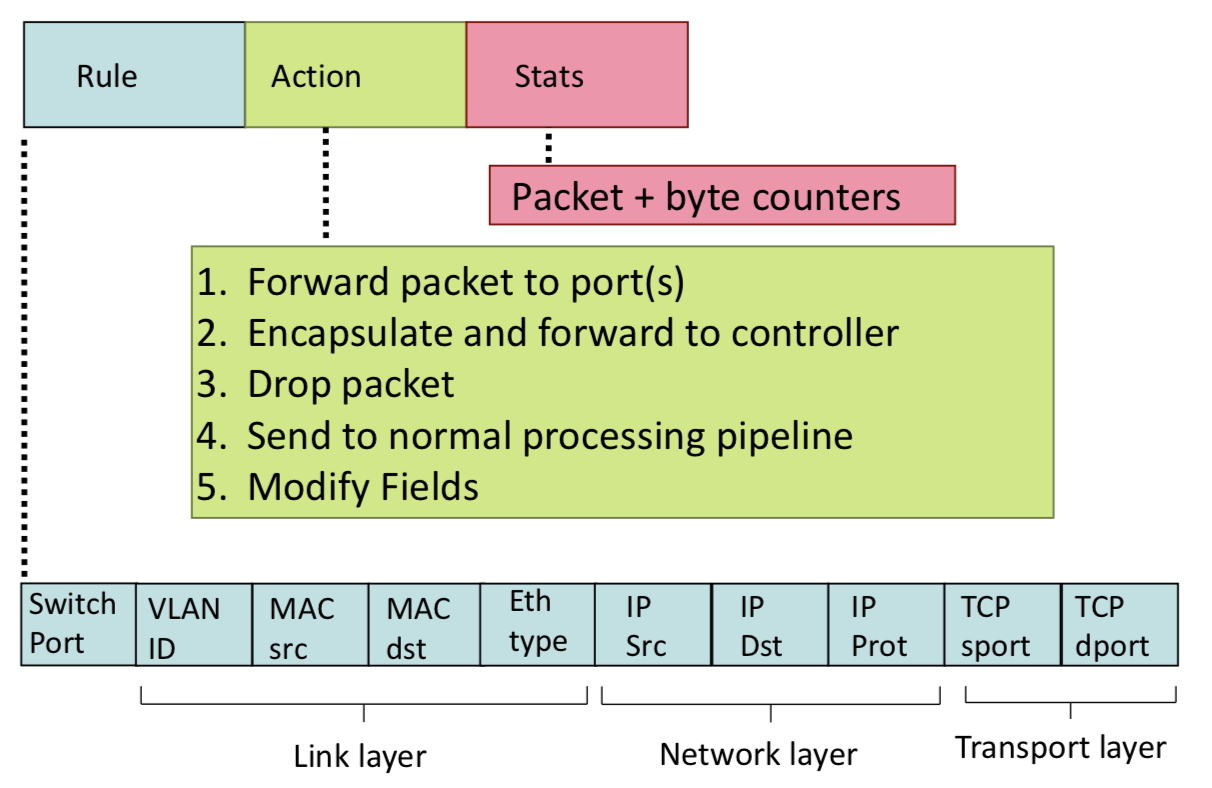
\includegraphics[width=\linewidth]{flow}
	\centering
	\caption{Flow Table Entries}
\end{figure}
\subsubsection{OpenFlow Abstraction}
\begin{itemize}
	\item \textbf{Match+Action:} unifies different kinds of devices
	\item Router
	\begin{description}
		\item[match:] longest destination IP prefix
		\item[action:] forward out a link
	\end{description}
	\item Switch
	\begin{description}
		\item[match:] destination MAC address
		\item[action:] forward or flood
	\end{description}
	\item Firewall
	\begin{description}
		\item[match:] IP addresses and TCP/UDP port numbers
		\item[action:] permit or deny
	\end{description}
	\item NAT
	\begin{description}
		\item[match:] IP address and port
		\item[action:] rewrite address and port
	\end{description}
\end{itemize}